\chapter{Background}
\label{sec:background}
\begin{itemize}
\item Introduction of relevant theory behind the thesis
\item In photorealistic, introduction to most relevant quantities, namely radiometric quantities, brdfs and bssrdfs. Scattering and non scattering media.
\item Offline and real time techniques. GPUs. 
\item ray tracign and rasterization. bleeding between the two.
\end{itemize}

\section{Photorealistic rendering}

\subsection{Radiometry}
Radiometry is that branch of science that measures electromagnetic radiation. We will define the basic radiometric quantities, in order to then introduce the two main reflectance functions of interest in this thesis, namely the BRDF and the BSSRDF. In particular, we want to give a definition of radiance, the most useful quantity in describing light transport along rays.

First, we consider an ideal point light source in space. The source emits a certain amount of energy $U$, measured in Joules $[J]$. The first quantity we derive is radiant flux or radiant power $\Phi$, defined as the amount of energy per second emitted by the light:
$$
\Phi = \frac{d U}{d t}  \siunit{\watt}.
$$
The radiant flux represents the overall power the light emits in all directions overall. We usually want to be more descriptive on how a light or a surface is emitting light, since not all the sources we consider are ideal. First, we are interested on how the light emission changes  We then define $I$ as radiant intensity, i.e. the amount of flux the light emits towards a specific direction $\vec{\omega}$:
$$
I(\vec{\omega}) = \frac{d \Phi}{d \omega}  \siunit{\watt \per \steradian}.
$$   
Where $d \omega$ is an infinitesimal solid angle around direction $\vec{\omega}$. An isotropic point light, by definition, as constant intensity across all directions.

We now consider a surface that receives light. In particular, we consider an infinitesimal oriented element of this surface $d \vec{A}$ around a point $\mathbf{x}$. The orientation of the surface is usually called the \emph{normal} and indicated by $\vec{n}$ We can now define irradiance as the amount of incoming flux received per unit area:
$$
E(\mathbf{x}) = \frac{d \Phi}{d A}  \siunit{\watt \per \square \metre}
$$
Similarly, we have a dual quantity for the flux \emph{emitted} by a unit element surface. We call this quantity \emph{radiosity} and we define it with the symbol $B$.
The most simple irradiance is the one emitted by an isotropic point light. In this case, the irradiance at a distance $R$ from the point light is 
$$
E = \frac{\Phi}{4 \pi R} \siunit{\watt \per \square \metre}
$$
So, the father we go from a point light, the less irradiance we receive, because the power $\Phi$ has to spread across a larger area.

Finally, we combine the definitions above into one, to define the last important basic radiometric quantity, \emph{radiance}:
$$
L(\mathbf{x}, \vec{\omega}) = \frac{d^2 \Phi}{d A \cos\theta d \omega}  \siunit{\watt \per \square \metre \per \steradian}
$$
Where $\cos \theta = \vec{n} \cdot \vec{\omega}$ is the cosine of the angle between the normal and the direction of evaluation. $d A \cos\theta$ is also called the \emph{projected area element}. As irradiance, radiance can be incoming or outgoing from a specific point. We indicate these quantities with $L_i$ and $L_o$, respectively. In graphics, radiance is usually the most useful quantity for two main reasons. First, the other quantities can be easily computed from radiance through radiometric integrals:
\begin{figure}
\centering
	 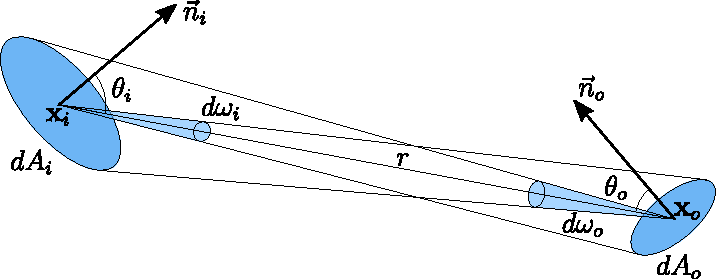
\includegraphics[scale=0.8]{figures/etendue}  \\
\caption{Configuration to prove the equality of radiance across a ray.} %The red rectangle shows where we estimated RMSE in Table \ref{table:quant}.}
\label{fig:etendue}
\end{figure}
\begin{equation*}
\begin{split}
\Phi &= \int_{\Omega} \int_{A} L(\mathbf{x}, \vec{\omega})  (\vec{n} \cdot \vec{\omega}) \ dA \ d \vec{\omega} \\
I(\vec{\omega}) &= \int_{A} L(\mathbf{x}, \vec{\omega})  (\vec{n} \cdot \vec{\omega}) \ dA  \\
E(\mathbf{x}) &= \int_{\Omega} L(\mathbf{x}, \vec{\omega})  (\vec{n} \cdot \vec{\omega}) \ d \vec{\omega} 
\end{split}
\end{equation*}
Where $\Omega$ and $A$ are the hemisphere around $\vec{n}$ and the total surface, respectively. Second, radiance carried by a ray \emph{in vacuo} is constant. We can prove this quite easily, with the aid of Figure\~ref{fig:etendue}. Note that for point $\mathbf{x}_o$, we have $d \omega_o = \frac{d A_i \cos\theta_i}{r^2}$, and dually the same for $\mathbf{x}_i$. Then:
\begin{equation*}
\begin{split}
L_i(\mathbf{x}_i, \vec{\omega}_i) = \frac{d^2 \Phi}{d A_i \cos\theta_i d \omega_i} &= 
\frac{d^2 \Phi}{d A_i \cos\theta_i \frac{d A_o \cos\theta_o}{r^2}}  
\\ &= \frac{d^2 \Phi}{\frac{d A_i \cos\theta_i}{r^2} d A_o \cos\theta_o } 
= \frac{d^2 \Phi}{d A_o \cos\theta_o d \omega_o} = L_o(\mathbf{x}_o, \vec{\omega}_o)
\end{split}
\end{equation*}

Note that we assume that the flux does not varies across the path, that is generally true if no objects are in the way and there is not medium in between the two points causing scattering events. 

\subsection{The BSSRDF and the BRDF}
So far, we have defined radiometric quantities, without worrying about the interaction at the surface. We will now describe how this radiometric quantities change once they encounter a surface. Let us first consider a surface illuminated by a light. Let us consider the portion of the flux $d \Phi_i$ arriving from direction $\vec{\omega}_i$ on a surface element $d A_i$ centered on a point $\mathbf{x}_i$. Due to surface interaction, part of the incoming light will emerge on a point $\mathbf{x}_o$, in direction $\vec{\omega}_o$. We consider the proportionality factor between the emitted radiance and the incoming flux:
$$
d L_o(\mathbf{x}_i, \vec{\omega}_i, \mathbf{x}_o, \vec{\omega}_o) = S(\mathbf{x}_i, \vec{\omega}_i, \mathbf{x}_o, \vec{\omega}_o) d \Phi_i(\mathbf{x}_i, \vec{\omega}_i)  \siunit{\watt \per \square \metre \per \steradian}
$$
The factor $S$, dependent on the surface materials, is called \emph{Bidirectional scattering-surface reflectance distribution function} (BSSRDF). The units for the BSSRDF are $\siunitnospace{\per \square \metre \per \steradian}$. From the definition of BSSRDF and flux, we obtain the extended form of the rendering equation:
$$
L_o(\mathbf{x}_o, \vec{\omega}_o) = \int_A \int_\Omega S(\mathbf{x}_i, \vec{\omega}_i, \mathbf{x}_o, \vec{\omega}_o) L_i(\mathbf{x}_i, \vec{\omega}_i) (\vec{n} \cdot \vec{\omega}_i) d A_i d \vec{\omega}_i  \siunit{\watt \per \square \metre \per \steradian}
$$
Note that we did not assume anything about the material, deriving the BSSRDF from purely radiometric quantities. Some simplifications can then be introduced to obtain more tractable functions. We assume that the BSSRDF is limited across a small area around the emergence point $\mathbf{x}_o$, and zero everywhere else. This is the case for a particular set of materials, such as plastic or metals. In this configuration, we can assume that the radiance is constant across the plane ($L_i(\mathbf{x}_i, \vec{\omega}_i) \approx L_i(\vec{\omega}_i)$). We also need to assume the material to be locally isotropic, i.e. its properties do not change across the surface. In this case, we can approximate the outgoing radiance as:
$$
d L_o(\mathbf{x}_o, \vec{\omega}_o) \approx \int_A d L_o(\mathbf{x}_i, \vec{\omega}_i, \mathbf{x}_o, \vec{\omega}_o) = \int_A S(\mathbf{x}_i, \vec{\omega}_i, \mathbf{x}_o, \vec{\omega}_o) d \Phi_i(\mathbf{x}_i, \vec{\omega}_i) 
$$
By the definition of flux, irradiance and the assumption of constant radiance:
\begin{equation*}
\begin{split}
d L_o(\mathbf{x}_o, \vec{\omega}_o) &\approx \int_A S(\mathbf{x}_i, \vec{\omega}_i, \mathbf{x}_o, \vec{\omega}_o) L_i(\mathbf{x}_i, \vec{\omega}_i) (\vec{n} \cdot \vec{\omega}_i) d A_i d \omega_i  \\ &= L_i(\vec{\omega}_i) (\vec{n} \cdot \vec{\omega}_i) d \omega_i \int_A S(\mathbf{x}_i, \vec{\omega}_i, \mathbf{x}_o, \vec{\omega}_o)   d A_i \\ &= d E_i(\vec{\omega}_i) \int_A S(\mathbf{x}_i, \vec{\omega}_i, \mathbf{x}_o, \vec{\omega}_o) d A_i
\end{split}
\end{equation*}
The last integral is a function purely dependent on the two angular vectors $\vec{\omega}_i$ and $\vec{\omega}_o$, and it becomes the proportionality constant between incoming irradiance and outgoing radiance:
$$
d L_o(\mathbf{x}_o, \vec{\omega}_o) = f_r(\mathbf{x}_o, \vec{\omega}_i, \vec{\omega}_o) d E_i(\mathbf{x}_o, \vec{\omega}_i)
$$
 The new function $f_r$ is called \emph{Bidirectional reflectance distribution function} (BRDF). The BRDF is measured in $\siunitnospace{\per \steradian}$. As before, we can obtain the outgoing radiance from the definition above:
$$
L_o(\mathbf{x}, \vec{\omega}) = \int_\Omega f_r(\mathbf{x}, \vec{\omega}_i,  \vec{\omega}_o) L_i(\mathbf{x}, \vec{\omega}_i) (\vec{n} \cdot \vec{\omega}_i) d\vec{\omega}_i  \siunit{\watt \per \square \metre \per \steradian}
$$
Which is the standard form of the rendering equation.

\subsection{Scattering media}
Scattering equation
Single terms: absorption, in scattering out scattering

\subsection{The BSSRDF}
Definition
Dipole configuration
Diffusion approximation
Example as the standard dipole

\subsection{Rendering techniques}
\fixme{Discuss with Jeppe whether to move in Related work?}
\begin{itemize}
\item The rendering equation
\item Path tracing
\item Rendering with reflectance functions
\end{itemize}

\section{Performance of rendering techniques} 

A comparison about rendering techniques. Offline vs realtime
Gpus vs cpus


\subsection{Offline rendering techniques}
Accuracy, slow rendering times. Focus on performance but mostly on achieving converged frames

\subsection{Real-time rendering techniques}
Disregard for physically based, but new interest in the lastest years

Squeezing as much as possible from the GPU. 



